\section{Laborgeräte und Werkzeuge}
Im Umgang mit Laborgeräten ergeben sich mehrere Fehlerquellen, welche in der Auswertung von Versuchen relevant sein können. Zu dem sollte jeweils der Nutzen des jeweiligen Arbeitsmittels bekannt sein, um Messungenauigkeiten zu vermeiden.



\subsection{Allgemeiner Apparaturaufbau}
Egal ob Umkristallisieren, Filtrieren oder Destillieren:\\
\begin{minipage}{0.45\textwidth}
	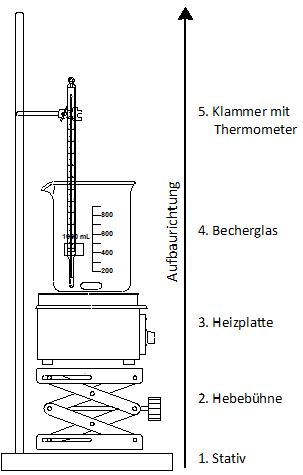
\includegraphics[width=0.8\textwidth]{img/Grundaufbau_Apparatur.png}
\end{minipage}
\begin{minipage}[b]{0.55\textwidth}
		 Im Regelfall sollte eine Apparatur von "`unten nach oben"' aufgebaut werden. Die Arbeitsweise sichert den Halt und erleichter das strukturierte Auf- und Abbauen der Apparatur.
\end{minipage}
\subsubsection{Klammern}

\subsubsection{Muffen}
\subsubsection{Stative}
\subsubsection{Korkringe}

\subsection{Volumengefäß}
\subsubsection{Bechergläser}
\subsubsection{Rundkolben}
\subsubsection{Erlenmeyerkolben}
\subsubsection{Maßkolben}
\subsubsection{Bürette}

\subsection{Pipetten}
\subsubsection{Peleusball}
\subsubsection{Vollpipetten}
\subsubsection{Eppendorfpipetten}
\subsubsection{Hubkolbenpipette}

\subsection{Trichter}
\subsubsection{Flüssigkeitstrichter}
\subsubsection{Feststofftrichter}
\subsubsection{Tropftrichter}
\subsubsection{Scheidetrichter}

\subsection{Schläuche}
\subsubsection{Vakuumschläuche}
\subsubsection{Wasserschläuche}
\subsubsection{Oliven}

\subsection{Filter}
\subsubsection{Filterpapier}
\subsubsection{Fritte}
\subsubsection{Filternutsche}

\subsection{Waschflaschen}

\subsection{Rührer}
\subsubsection{Magnetrührwerk}
\subsubsection{Rührertypen}
\subsubsection{Rührermotor}

\subsection{Rückflusskühler}
\subsubsection{Dimrothkühler}
\subsubsection{Liebigkühler}

\subsection{Heizelemente}
\subsubsection{Wärmebad}
\subsubsection{Brenner}
\subsubsection{Heizpilz oder Heiznetz}
\subsubsection{Heizplatte}

\subsection{Pyknometer}

\subsubsection{Apparaturen zum Trocknen}
\subsubsection{Exsikkator}
\subsubsection{Trockenschrank}
\subsubsection{Muffelofen}

\subsection{Pumpen}
\subsubsection{Vakuumpumpe (Wasserstrahlpumpe)}
\subsubsection{Hubkolbenpumpe}
\subsubsection{Kreiselpumpe}

\subsection{Zusätzlich:}
\subsubsection{Beschriftung von Proben}
\subsection{Füllkörper}
\subsubsection{Schliffe und Schlifffett}
\subsubsection{Ultraschallbad}
\subsubsection{Eismaschine}